Après vous avoir introduit le contexte du projet, nous allons maintenant vous expliquer comment nous avons fait pour implémenter le crypto-système RSA sur un firmware customisé de la ChipWhisperer.

\subsection{Implémentation sur 32 bits}
Dans un premier temps, nous avons décidé d'implémenter le RSA sur des petits nombres de taille supportés nativement par le crypto-processeur. Ce dernier utilise une architecture de 32 bits, cela signifie que lorsqu'on stock un nombre dessus, ce nombre ne peut être que de 32 bits maximum (de $0$ à $2^{32} - 1$, pour des entiers positifs). Nous allons donc commencer par implémenter le RSA sur des nombres de 32 bits afin de pouvoir utiliser les opérations usuelles : addition, multiplication, réduction modulaire, ...\\

Comme nous l'avons vu dans la section précédente, pour implémenter le RSA, nous avons besoin de savoir trois choses différentes :
\begin{enumerate}
	\item Générer des clés de chiffrement/déchiffrement ;
	\item Chiffrer un message $m$, sur 32 bits $m < 2^{32}$;
	\item Déchiffrer un chiffré $c$, sur 32 bits $c < 2^{32}$.
\end{enumerate}

Les algorithmes nécessaire pour effectuer ces opérations sont : la génération de nombres premiers aléatoire afin de déterminer $p$ et $q$, le calcul d'inverse modulaire pour déterminer la clé privée $d$ tel que $ed \equiv 1 [n]$ et l'exponentiation modulaire afin de chiffrer et déchiffrer, cf. équation (\ref{eq:chiffrement}) et (\ref{eq:dechiffrement}).\\

Nous avons écrit le pseudo-code des ces deux algorithmes essentiels (cf. Algorithme \ref{alg:expomod} et \ref{alg:invmod}), pour ce qui est de leur implémentation en C dans le firmware de la ChipWhisperer, vous pouvez les retrouver dans l'archive finale du projet.

\medskip
\begin{algorithm}[p]
\SetAlgoLined
\KwIn{base, exponent, modulus}
\KwOut{result}
$result \leftarrow 1$\;
$base \leftarrow base \mod modulus$\;
\While{$exponent > 0$}{
  \If{$exponent$ est impair}{
    $result \leftarrow (result \times base) \mod modulus$\;
  }
  $exponent \leftarrow exponent \div 2$\;
  $base \leftarrow (base \times base) \mod modulus$\;
}
\KwRet{$result$}\;
\caption{Pseudo-code de l'exponentiation modulaire}
\label{alg:expomod}
\end{algorithm}
\medskip

\begin{algorithm}[p]
\SetAlgoLined
\KwIn{a, m}
\KwOut{inverse modulaire}
$m0 \leftarrow m$\;
$y \leftarrow 0$\;
$x \leftarrow 1$\;
\If{$m = 1$}{
  \KwRet{$0$}\;
}
\While{$a > 1$}{
  $q \leftarrow a \div m$\;
  $t \leftarrow m$\;
  $m \leftarrow a \mod m$\;
  $a \leftarrow t$\;
  $t \leftarrow y$\;
  $y \leftarrow x - q \times y$\;
  $x \leftarrow t$\;
}
\If{$x < 0$}{
  $x \leftarrow x + m0$\;
}
\KwRet{$x$}\;
\caption{Pseudo-code de l'inverse modulaire}
\label{alg:invmod}
\end{algorithm}

% Nous pouvons voir que pour le premier algorithme, celui d'exponentiation rapide modulaire, nous utilisons un algorithme efficace contrairement à l'algorithme naïf qui consisterait a faire : $\underbrace{x \times x \times \ldots \times x}_{\text{n fois}}$. Afin de mettre en valeur la différence de complexité entre ces deux version, vous pouvez retrouver Figure \ref{fig:diff_complexite} la graphe représentant le nombre d'opération requis en fonction de l'exposant.
% \begin{figure}[H]
%     \centering
%     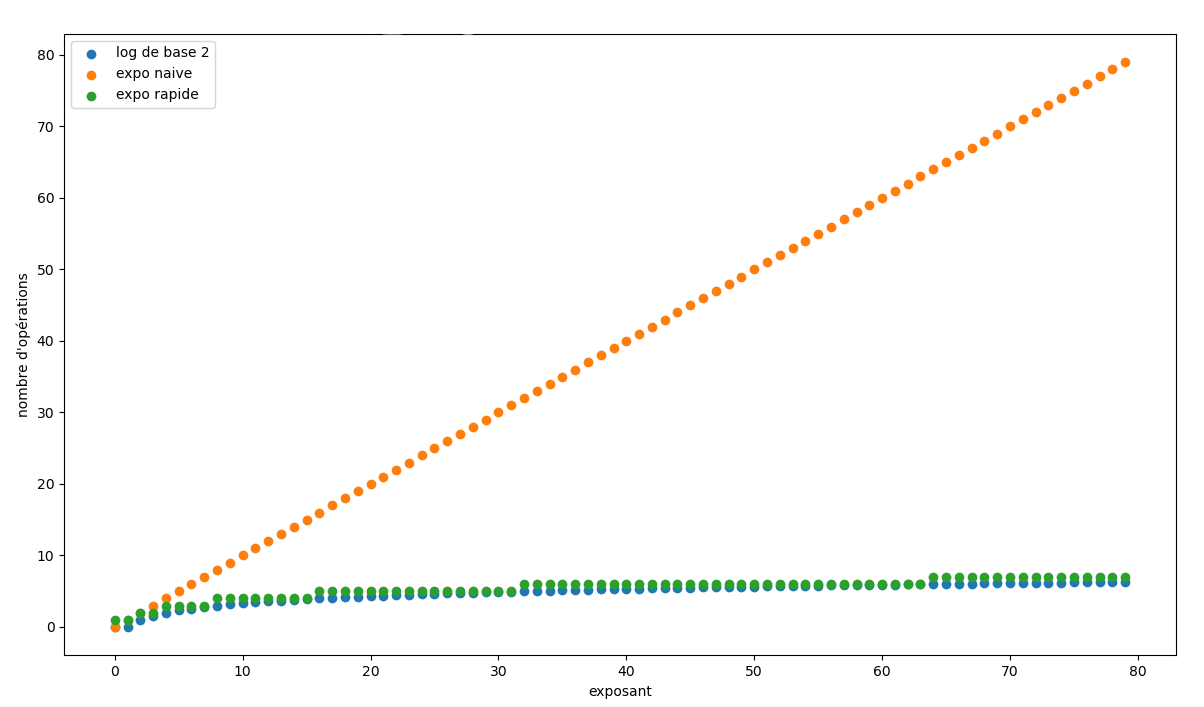
\includegraphics[width=\textwidth]{fig/diff_complexite.png}
%     \caption{Comparaison des complexités des deux algorithmes d'exponentiation}
%     \label{fig:diff_complexite}
% \end{figure}
% Il est aussi important de relever que la présence de l'algorithme d’exponentiation rapide n'est pas un hasard, c'est grâce à lui que le système est faillible. En effet, si il rencontre un $1$ dans la représentation binaire du nombre il fait 2 calculs, sinon, il en fait 1 seul. Grâce à ça, il a une fuite de la clé qui s’opèrera sur la trace de consommation électrique.

% Notre implémentation en C de ces deux algorithmes se trouve dans l'archive final du projet. Une fois ces primitives implémentées, il a été facile d'implémenter la génération de clé, le chiffrement et le déchiffrement, vous pouvez également retrouver ces implémentations en C dans l'archive final du projet.

\subsection{Objectif 2048 bits}
D'après les recommandation de l'ANSSI \cite{anssi:guide}, un RSA implémenté avec les types de bases du C ($32$ bits), n'est pas du tout sécurisé. En effet, nous pouvons retrouver page 19 les règles suivantes :
\begin{enumerate}
  \item La taille minimale du module est de $2048$ bits, pour une utilisation ne devant
pas dépasser la fin de l’année 2030.
  \item Pour une utilisation à partir de l’année 2031, la taille minimale du module
est de $3072$ bits.
  \item Les exposants secrets doivent être de même taille que le module.
  \item Pour les applications de chiffrement, les exposants publics doivent être strictement supérieurs à $2^{16} = 65536$.
\end{enumerate}
Afin d'attaquer une version du RSA qui pourrait être utilisé dans un cadre réel, nous allons donc devoir l'implémenter avec un module, notée $n$ précédemment, de 2048 bits ! Or, comme vu précédemment nous allons utiliser une machine en 32 bits, ce qui signifie que les types de bases sur lesquels les opérations élémentaires sont implémentées, ne dépasse pas 32 bits. Nous allons devoir créer et implémenter des opérations sur les grands nombres, nous appellerons BigInt ces derniers dans le reste du rapport car c'est l'usage.

\subsection{Implémentation du big int}
Pour représenter un grand entier dans un système embarqué 32 bits, nous utilisons un découpage en chunks de 16 bits. Imaginons que nous souhaitons un nombre de 64 bits. Nous divisons cet entier en mots de 16 bits. Ainsi, chaque chunk de 16 bits contient une partie du grand entier.\\

Prenons un exemple concret : supposons que notre grand entier soit \texttt{0xABCD1234567890EF}. Pour le découper en chunks de 16 bits, nous aurons :

\begin{itemize}
\item Chunk 1: \texttt{0xABCD}
\item Chunk 2: \texttt{0x1234}
\item Chunk 3: \texttt{0x5678}
\item Chunk 4: \texttt{0x90EF}
\end{itemize}

Chaque chunk peut être représenté par un entier de 16 bits dans la mémoire du système embarqué. En utilisant cette méthode de découpage, nous pouvons stocker et manipuler des grands entiers même dans des systèmes avec des limitations de taille de données.\\

Si nous utilisons des sous-entiers de 16 bits et pas de 32 bits c'est parce que le 32 bits servira de type d'overflow, en effet lorsqu'on aura une sous opération qui dépassera la taille d'un chunk alors un entier de 32 bits permettra de résoudre ce problème.\\

Sachant que chaque chunk est sur $16$ bits c'est comme si nous avons une représentation du nombre en base $2^{16}$, nous n'avons ``plus'' qu'a considéré un chunk comme un symbole de la base $2^{16}$ et implémenté les opérations usuelles dessus.\\

Cette méthode fonctionne pour l'addition et la soustraction, mais pour les opérations d'inverse modulaire, de multiplication modulaire et de division, cela ne fonctionne plus et il faut utiliser des algorithmes plus poussés, nous nous sommes basé sur ceux du livre ``Handbook of Applied Cryptography'' \cite{hac:ch14}.
\subsection{Conclusion}
